\documentclass[a4paper]{article}
\usepackage[14pt]{extsizes} % для того чтобы задать нестандартный 12-ый размер шри
\usepackage[left=20mm, top=15mm, right=15mm, bottom=15mm, nohead, footskip=10mm]{geometry} % настройки полей документа
\usepackage{wrapfig}
\usepackage{placeins} 
\usepackage{hyperref}
\usepackage[warn]{mathtext}
\usepackage[utf8]{inputenc}
\usepackage{amsmath,amsfonts,amssymb,amsthm,mathtools}
\usepackage[russian]{babel}
\usepackage{graphicx}
\usepackage[shortcuts,cyremdash]{extdash}
\usepackage{floatflt}
\usepackage{lipsum}
\usepackage{verbatim}
\usepackage{concmath}
\usepackage{euler}
\usepackage{xcolor}
\usepackage{etoolbox}
\usepackage{subfiles}
\usepackage{enumitem}
\usepackage{import}
%\usepackage{autonum}
\graphicspath{}
\DeclareGraphicsExtensions{.pdf,.png,.jpg}
\usepackage{graphicx}

%\DeclareMathOperator{\sign}{sign}


\newcommand{\image}[3]
{
	\begin{figure}[h]
		\center{\includegraphics[scale=#2]{#1}}
		\caption{#3}
	\end{figure}
}

\RequirePackage{caption2}
	
\newcommand*{\hm}[1]{#1\nobreak\discretionary{}
	
	\DeclareSymbolFont{T2Aletters}{T2A}{cmr}{m}{it}
	
	{\hbox{$\mathsurround=0pt #1$}}{}}
	
% Цвета для гиперссылок
\definecolor{linkcolor}{HTML}{0000FF} % цвет ссылок
\definecolor{urlcolor}{HTML}{799B03} % цвет гиперссылок

\hypersetup{pdfstartview=FitH,  linkcolor=linkcolor,urlcolor=urlcolor, colorlinks=true}

\begin{document}% начало документа
% НАЧАЛО ТИТУЛЬНОГО ЛИСТА
\begin{center}
	\hfill \break
	\hfill \break
	{\small ФЕДЕРАЛЬНОЕ ГОСУДАРСТВЕННОЕ АВТОНОМНОЕ ОБРАЗОВАТЕЛЬНОЕ\\ УЧРЕЖДЕНИЕ ВЫСШЕГО ОБРАЗОВАНИЯ\\ МОСКОВСКИЙ ФИЗИКО-ТЕХНИЧЕСКИЙ ИНСТИТУТ\\ (НАЦИОНАЛЬНЫЙ ИССЛЕДОВАТЕЛЬСКИЙ УНИВЕРСИТЕТ)\\ ФИЗТЕХ-ШКОЛА РАДИОТЕХНИКИ И КОМПЬЮТЕРНЫХ ТЕХНОЛОГИЙ}\\

	\hfill \break
	\normalsize{ВОПРОС ПО ВЫБОРУ ПО ОБЩЕЙ ФИЗИКЕ}\\
	\vspace{7em}
	\normalsize{\textbf{По теме}}\\
	\vspace{7em}
	\large{<<Квазистатическое соударение шаров. Теория Герца>>}\\
\end{center}

\vspace{16em}
\begin{flushright}
	\normalsize{Студента 1 курса группы Б01-003}\\
	\normalsize{\textbf{Крейнина Матвея Вадимовича}}\\
\end{flushright}

\vspace{\fill}
\begin{center}
	\normalsize{\textbf{Долгопрудный, 2020}}
\end{center}


\thispagestyle{empty} % выключаем отображение номера для этой страницы

% КОНЕЦ ТИТУЛЬНОГО ЛИСТА

\newpage
\tableofcontents
\newpage

\section{Классическая теория абсолютно упругого удара}


Предлагаю вспомнить, что называют абсолютно упругим ударом -- это удар, в результате которого не меняются внутренние состояния сталкивающихся тел и, соответственно, их внутренние энергии. Тогда наряду с суммарным импульсом тел сохраняется также их суммарная кинетическая энергия. Эти два закона сохранения и позволяют однозначно определить скорости тел после лобового удара по известным значениям скоростей до него. В дальнейшем я буду рассматривать одинаковые шары, налетающие друг на друга с одинаковыми скоростями V. Если бы мы могли считать удар абсолютно упругим, то шары просто разлетелись бы с точно такими же скоростями. Теперь я предлагаю разобраться, что происходит в действительности.

\section{Отклонения от абсолютной упругости}
В реальной жизни идеальный абсолютно упругий удар не встречается, также как и другие идеалы. При реальном ударе часть $\delta W$ начальной кинетической энергии $W = mv^2$ переходит в тепло и теряется. Следовательно, упругость удара можно было бы считать абсолютной при $\delta W/W = 0$, а при $\delta W/W \ll 1$ разумно надеяться, что удар можно считать абсолютно упругим приближенно.
Предлагаю качественно оценить, что происходит во время удара. При столкновении шары сначала приходят в соприкосновение в одной точке, затем, продолжая по инерции сближаться, они все больше деформируют друг друга, соответсвующая упругая сила растет и сообщает каждому из шаров растущее по абсолютной величине отрицательное ускорение -- и так до того момента, как они остановятся. После этого скорости поменяют свой знак и шары начнут расходиться, упругие деформации будут уменьшаться, и тела разлетаются в разные стороны. 
\begin{center}
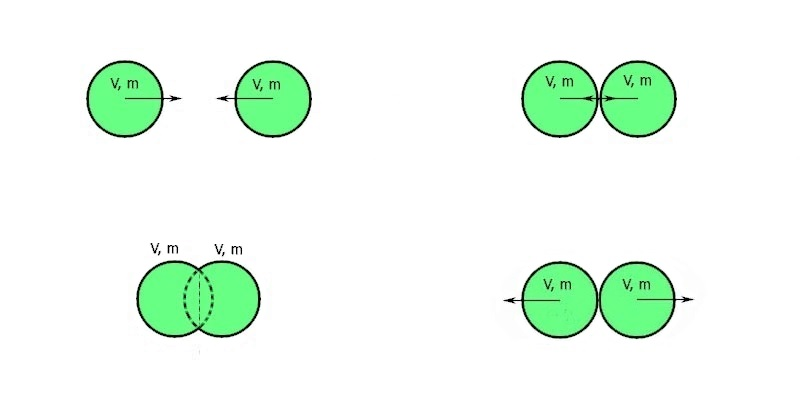
\includegraphics[scale=0.7]{vpv-image1.jpg}
\end{center}
\section{Причины потери энергии}
Каковы же причины потери энергии? Например, если эти шары не являются абсолютно упругими, то при деформации происходит выделение тепла, т.е. уменьшается механическая энергия. Но, если шары были бы абсолютно упругими, то удар все равно не был бы абсолютно упругим. Энергия может переходить в колебания внутри шаров после их разлета. Или, более точно, в виде звуковых волн, которые возбуждаются при ударе и продолжают бегать по каждому шару, отражаясь от его границ после того, как сам удар закончится.


Обычно в реальной жизни скорость шаров гораздо меньше скорости звука $s$ (скорость звука в материале, из которого сделаны шары). Предположим, что параметр $\frac{\delta W}{W}$ как-то связан с отношением $v/s$. В частности, если мы будем анализировать случай практически упругого удара с $\frac{\delta W}{W} \ll 1$, то должны считать, что $v/s \ll 1$. Начнем со статической деформации друг друга, когда шары обладают нулевой скоростью и статически деформируют друг друга.
\section{Статическая деформация упругого удара}
Допустим, что два шара одного и того же радиуса $R$ сдавлены друг с другом некоторой постоянной силой $F$ так, что их центры сближены до расстояния $2(R-h)$. Надо выяснить как зависит сила $F$ от $h$.
Шары контактируют друг с другом по некоторой плоской площадке. Эта система имеет ось симметри - прямую, соединяющую центры шаров. Из этого можно сделать вывод, что площадка контакта представляет собой круг. Обозначим его радиус за a. Предположим, что поверхность каждого из шаров остается сферической, за исключением плоской площадки контакта. Тогда применим теорему пифагора к треугольнику $\vartriangle OAB$, что нам даст 
$(R-h)^2+a^2=R^2$
или же 
$a^2-2Rh+h^2=0$
т.е. если сжатие у нас слабое и $h \ll R$ и вторым порядком малости можно пренебречь ($h^2$) получаем, что $a = \sqrt{2Rh}$
Но на самом деле вблизи площадки контакта поверхности отклоняются от сферических, поэтому мой ответ для a несколько завышенный. Но поскольку меня интересует только оценка, а не точный коэффециент, то получаю, что

\begin{equation}
a \sim \sqrt{Rh}.
\label{eq1}
\end{equation}

\begin{center}
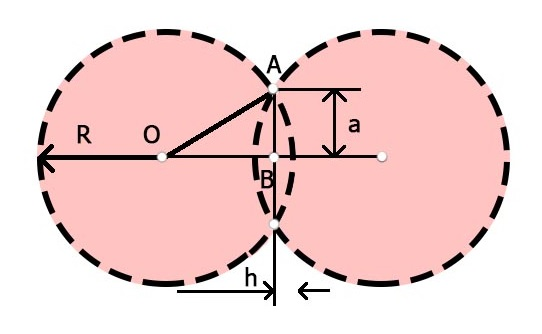
\includegraphics[scale=0.5]{vpv-image.jpg}
\end{center}
Также запомним, что для $h \ll R$ получается $a \gg h$.


Логичное предположение, что вдали от площадки контакта материал остается недеформированным, а деформация проходит в глубь тела на расстояние $\sim a$. Область, где локализованы все деформации, не имеет, очевидно, четкой границы, но она имеет площадь поперечного сечений $\sim a^2$ и длину $\sim a$. Следовательно, искомую силу можно оценить с помощью закона Гука:
$F = k \frac{\Delta l }{l}$. 
Абсолютная деформация $\Delta l \sim h$, недеформированный размер $l \sim a$, постоянная упругости пропорциональна поперечному сечению деформированного тела, т.е. $k \sim Ea^2$, где $E$ - модуль упругости материала, из которого сделаны шары. Следовательно можно сделать вывод, что: 
\begin{equation}
F \sim E a^2 \frac{h}{a} \sim E h^{\frac{3}{2}} R^{\frac{1}{2}}
\label{eq2}
\end{equation}
Эта зависимость была найдена Герцем в 1887 году. Особенность формулы Герца в том, что сила упругости не пропорциональна деформации. С ростом h сила растет как $h^{\frac{3}{2}}$. Это вполне логично, ведь с ростом $h$ деформированию сопротивляется все более широкий участок каждого из шаров.
\\
Зная выражение для силы $F(h)$ можно легко оценить потенциальную энергию деформирования $U(h)$. Она в точности равна работе, которую сила F производит над телами, увеличивая деформацию от нуля до h, т.е.
\begin{equation}
U(h) \sim F(h)h \sim Eh^{\frac{5}{2}}R^{\frac{1}{2}}
\label{eq3}
\end{equation}
Или же интегарл от:
\begin{equation}
U(h)=\int\limits_0^h F(x)\,dx
\label{eq4}
\end{equation}

\section{Квазистатические представления об ударе}
От неподвижных сдавленных тел вернемся к сталкивающимся и рассмотрим момент максимальной деформации, когда тела остановились на мгновение перед тем, как начать разгон в обратную сторону. В этот момент вся кинетическая энергия двух шаров $mv^2$ превращена в потенциальную энергию деформации. Следовательно, максимальное сближение шаров при ударе можно оценить с помощью формулы (\ref{eq3}): так как для одного шара $U(h_{макс})=\frac{mv^2}{2}, то$
\begin{equation}
h_{макс} \sim v^{\frac{4}{5}}m^{\frac{2}{5}}R^{\frac{-1}{5}}E^{\frac{-2}{5}}
\label{eq5}
\end{equation}
Эту формулу можно записать в более красивом виде, если заметим, что величина:
\begin{equation}
s \sim E^{\frac{1}{2}}\left(\frac{m}{R^3}\right)^{\frac{-1}{2}}
\label{eq6}
\end{equation} 
это скорость звука в материале шаров. Можно подтвердить из соображений размерности. Подобно тому, как частота колебаний груза на пружине $\sqrt{\frac{k}{m}}$ зависит от жесткости $k$ и массы $m$, скорость звука $s$ должна зависеть от <<жесткости>> (модуля упругости) материала $E$ и его плотности $\rho$. $E$ имеет размерность давления, т.е. это сила, деленная на площадь, или же масса деленная на длину и квадрат времени, плотность это масса, деленная на объём. Составить размерность скорости из этих величин можно едиственным способом:
\begin{equation}
s \sim \sqrt{\frac{E}{\rho}}
\label{eq7}
\end{equation}
Т.к. для шара $\rho = \frac{m}{\frac{4}{3} \pi R^3} \sim \frac{m}{R^3}$
откуда можно получить оценку (\ref{eq6}). Используя эти оценки предлагаю переписать (\ref{eq5})
\begin{equation}
h_{макс} \sim R\left(\frac{v}{s}\right)^{\frac{4}{5}}
\label{eq8}
\end{equation}
Получившаяся формула очевидна своим физическим смыслом: при медленном столкновении, когда $\frac{v}{s} \ll 1$, т.е. скорость шаров мала по сравнению со скоростью звука, деформация, даже максимальная, остается маленькой во времся всего столкновения:
$h_{макс} \ll R.$ Это удовлетворяет ранее упоминавшейся качественной оценке того, что удар близок к абсолютно упругому при $v \ll s.$


Легко оценить и время столкновения $\tau$: это время, в течение которого тела будут оставаться в контакте, успевая пройти путь $\sim h_{макс}$.
Поскольку средняя скорость на пути от первого соприкосновения до остановки $\sim v$, то получается, что:
\begin{equation}
\tau \sim \frac{h_{макс}}{Rv^{\frac{-1}{5}}s^{\frac{-4}{5}}}
\label{eq9}
\end{equation}
\newline
Формулы (\ref{eq8}) и (\ref{eq9}), также как и (\ref{eq2}), и (\ref{eq3}), принадлежат Герцу.
\newline

\section{Оценка динамических величин}
Максимальная деформация $h_{макс}$ достигается за сравнительно короткое время $\tau$. Быстрое деформирование создает в телах звуковые волны, и можно сказать, что эти волны несут каждой точке шара <<сообщение>> о том, какие деформации и напряжение должны в ней устанавливаться. В упругом теле с малым внутренним трением звуковые волны очень медленно затухают. Поэтому статическое распределение деформаций и напряжений в материале может установиться после того, как звук успеет много раз обежать всю внутренность шара, отражаясь от поверхности. В частности, такое время должно пройти, чтобы упругая сила действующая со стороны шара на партнера, приблизилась к своему статическому значению (\ref{eq2}). Следовательно мои оценки имеют шанс быть тривиальными при условии $\tau \ll \frac{R}{s}$, где $\frac{R}{s}$ - время необходимое звук, чтобы пройти сквозь шар один раз. Вспоминая оценку (\ref{eq9}) величины $\tau$, получаем из неё же условие её применимости:
\begin{equation}
v^{\frac{-1}{5}}s^{\frac{1}{5}} \gg 1, \text{ или же } \frac{v}{s} \ll 1
\label{eq10}
\end{equation}
Можно подумать, что странно выводить из самой формулы границы ей применимости, но нет, здесь всё в порядке. Если $\frac{v}{s} \ll 1$, то заложенное в основу формулы (\ref{eq9}) преположение о многократном обегании шара звуком ей не противоречит и, значит, формула применима. 


Условие $\frac{v}{s} \ll 1$ - единственное условие применимости всех моих построений: оно гарантирует малость деформаций $h \ll R$ в течение всего процесса, и оно же обеспечивает применимость квазистатического подхода, т.е. использования статических формул для упругой или потенциальной энергии.

\section{Заключение}
Если бы я начал оценивать потерю энергии $\delta W$, то это потребовало бы выхода в другую область физики - колебания, вместо относительно простой статической упругости. Если бы речь зашла о другом предельном случае $\frac{v}{s} \gg 1$, то это потребовало перехода в разрушение, хрупкость и пластичность, или же если $v \cong c$, то это уже будет физика столкновений тяжелых ионов. Поэтому это условие является крайне важным в данной работе. Если же $v \cong s$, то данная модель уже не будет применима и придется учитывать колебания, которая возникают внутри шаров и потерю энергии. 

\section{Источники}
<<Повесть о том, как столкнулись два шара, или что такое малый параметр>> А. Гроссберг
\end{document}